\documentclass[11pt,a4paper]{article}
\usepackage[ngerman]{babel}
\usepackage[T1]{fontenc}
\usepackage[utf8]{inputenc}
\usepackage[margin=2.2cm]{geometry}
\usepackage{lmodern}
\usepackage{tikz}
\usepackage{graphicx}
\usepackage{booktabs}
\usepackage{array}
\usepackage{fancyvrb}
\usepackage{listings}
\usepackage{xcolor}
\usepackage{float}
\usepackage{hyperref}

\lstset{basicstyle=\ttfamily\footnotesize, frame=single, columns=fullflexible,
        keywordstyle=\color{blue}\bfseries, commentstyle=\color{green!50!black}}
\lstdefinelanguage{SV}{morekeywords={module,endmodule,input,output,logic,always_comb,
        begin,end,case,endcase,default,assign}, morecomment=[l]{//}}

        
\title{Assignment 01 -- Seven Segment Decoder\\\large EIT HDL -- Doku}
\author{Lukas Wolf}
\date{\today}

\begin{document}
\maketitle

\section{Aufgabe}
Das Modul \texttt{sevenseg} übersetzt eine 4-Bit-Binärzahl \texttt{bin\_i[3:0]} in das
Segmentmuster \texttt{hex\_o[6:0]} einer Siebensegmentanzeige. Zusätzlich liefert \texttt{hexn\_o[6:0]} das
negierte Muster für Low-aktive Anzeigen.

\section{Implementierung}
Der Decoder ist als Verhaltensbeschreibung in einem \texttt{always\_comb}-Block mit einer
\texttt{case}-Anweisung umgesetzt. Am Ende wird \texttt{hexn\_o} negiert.

\begin{lstlisting}[language=SV]
always_comb begin
    case (bin_i)          
        4'h0   : hex_o = 7'b0111111;
        4'h1   : hex_o = 7'b0000110;
        ...
        4'hF   : hex_o = 7'b1110001;
        default: hex_o = 7'b0000000; 
    endcase
end

assign hexn_o = ~hex_o;
\end{lstlisting}

\section{Verifikation}
Die Testbench legt alle 16 Eingangswerte im Abstand von 100\,ns an, gibt Ein- und Ausgänge
mit \texttt{\$display} in der Konsole aus. Die Ausgaben werden anschließend mit Figure~3 der
Angabe verglichen. Gestartet wird die Simulation in ModelSim mit
\texttt{do sim\_tb\_sevenseg.tcl}. Das Skript öffnet das Wave-Fenster mit allen relevanten
Signalen (Testbench-Signale, DUT-Ports und die Einzelbits von hex\_o).

\subsection*{Simulator-Ausgabe}
\VerbatimInput[fontsize=\scriptsize, frame=single]{transcript.txt}

\subsection*{Wave-Fenster}
\begin{figure}[H]\centering
  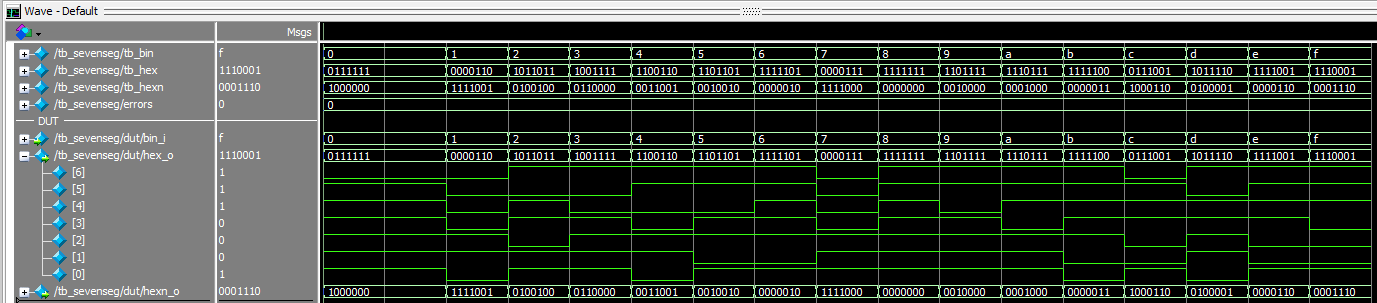
\includegraphics[width=\linewidth]{modelsim.png}
  \caption{ModelSim Wave-Fenster der Simulation von \texttt{tb\_sevenseg}.}
\end{figure}

\paragraph{Ergebnis} Alle 16 Eingangskombinationen liefern das erwartete Muster,
hexn\_o ist in jedem Fall die bitweise Negation von hex\_o.
Das Modul erfüllt damit die Spezifikation.

\section{Diskussion der Implementierungsart}
\begin{tabular}{>{\raggedright}p{3.4cm}>{\raggedright}p{5.8cm}>{\raggedright\arraybackslash}p{5.8cm}}
\toprule
Methode & Vorteile & Nachteile \\ \midrule
Gatter (\texttt{and}, \texttt{or}, \dots) &
Man bestimmt jedes einzelne Gatter selbst. &
Für 7 Segmente braucht man sehr viele Gatter. Das ist viel Arbeit, man macht leicht
Fehler und der Code ist schwer zu lesen. \\[1mm]
\texttt{assign} mit Formeln &
Kurzer Code. &
Schwierig zu lesen und nachzuvollziehen. \\[1mm]
\textbf{\texttt{always\_comb} mit \texttt{case}} (gewählt) &
Code ist leicht zu lesen und zu ändern. &
Etwas mehr Zeilen Code. \\
\bottomrule
\end{tabular}

\medskip

\end{document}
